The m-file \texttt{heat\_CN.m} solves the heat equation $u_t = \kappa u_{xx}$ using the Crank-Nicolson method. Run this
code, and by changing the number of grid points, confirm that it is second-order accurate. (Observe how the error at
some fixed time such as $T = 1$ behaves as $k$ and $h$ go to zero with a fixed relation between $k$ and $h$, such as
$k = 4h$.)

\begin{solution}\ \\\\
    To verify second-order accuracy, we let $k = 4h$ (i.e., $\alpha = 4$); the output of \texttt{problem\_2a.m} is 
    given below:

    \begin{figure}[h]
        \centering
        \begin{verbatim}
                 h            k          error
            5.0000e-02   2.0000e-01   8.3163e-04
            3.3333e-02   1.3333e-01   2.6327e-04
            2.5000e-02   1.0000e-01   1.5711e-04
            2.0000e-02   8.0000e-02   9.7091e-05
            1.0000e-02   4.0000e-02   2.5266e-05
          
         Least squares fit gives E(h) = 0.421658 * h^2.12875
        \end{verbatim}
        \caption{Output of \texttt{problem\_2a.m}}
    \end{figure}
    
    \begin{figure*}[h]
        \centering
        \begin{subfigure}[b]{0.475\textwidth}
            \centering
            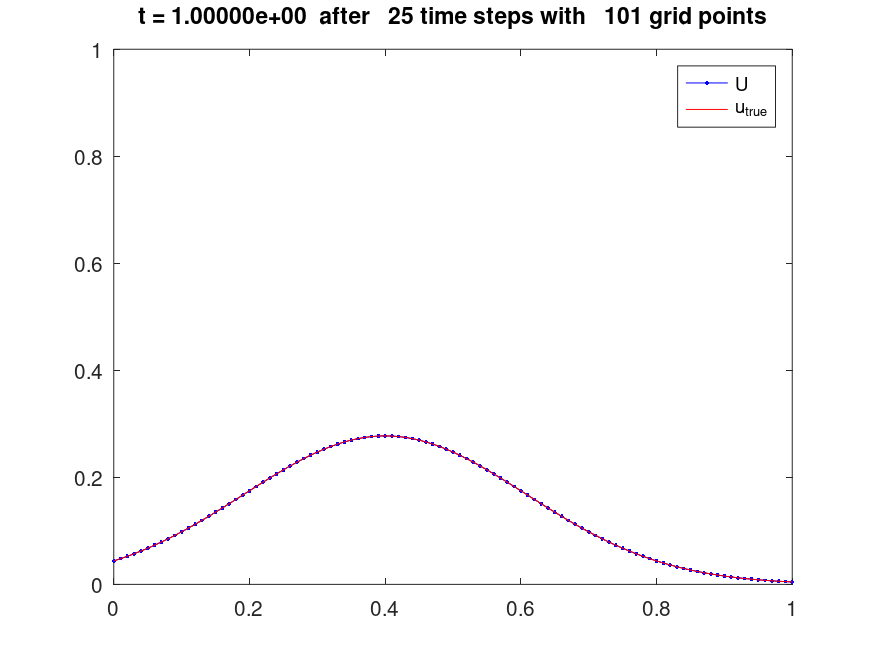
\includegraphics[width=\textwidth]{problem_2a_heatCN_t-25.png}
            \caption{CN method for $m = 99$ at $t = 1$}
        \end{subfigure}
        \hfill
        \begin{subfigure}[b]{0.475\textwidth}
            \centering
            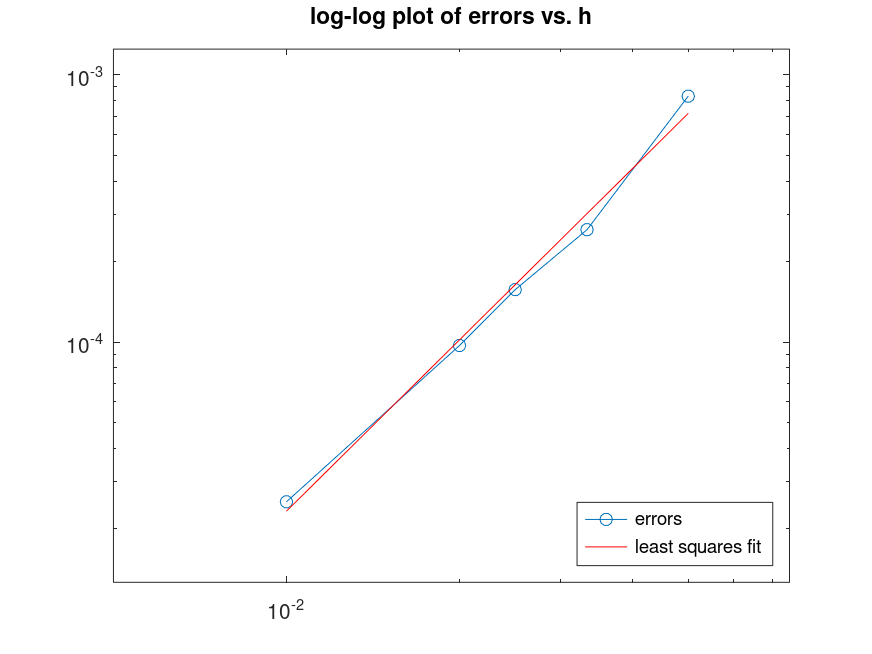
\includegraphics[width=\textwidth]{problem_2a_heatCN_error.png}
            \caption{CN error}
        \end{subfigure}
        \caption[]{Crank-Nicolson solution}
    \end{figure*}

    The least squares fit from above corresponds to $h$ versus error, and because \linebreak
    $\Delta t = k = 4h = 4 \Delta x$, we see that the Crank-Nicolson method is indeed \linebreak
    $\mathcal{O}\left(h^2 + k^2\right)$, as desired.
    \ \\
\end{solution}